\documentclass[12pt, a4paper]{article}

\usepackage[brazil]{babel} % section and appendix headings in Portuguese
\usepackage{setspace} % line spacing
\usepackage{times} % font times new roman
\usepackage[bottom=2cm,top=3cm,left=3cm,right=2cm]{geometry} % margins ABNT
\usepackage{ragged2e} % justified text
\usepackage{graphicx} % figures
\usepackage{float} % position of contents right after text
\usepackage{subcaption}  % subcaptions for figures, tables etc
\usepackage{caption} % captions for figures, tables etc
\usepackage{hyperref} % hyperlinks for references, figures and tables
\usepackage{multirow} % multirow tables
\usepackage[alf,abnt-repeated-title-omit=yes,abnt-emphasize=bf,abnt-full-initials=no]{abntex2cite}
\citebrackets() % parenthesis brackets for citations
\setlength\parindent{0pt} % no indentation
% \renewcommand{\citeonline}{#1}

\setcounter{secnumdepth}{5} % section numbering depth
\setcounter{tocdepth}{5} % table of contents depth

\def\changemargin#1#2{\list{}{\rightmargin#2\leftmargin#1}\item[]} % paragraph margin adjustment
\let\endchangemargin=\endlist % paragraph margin adjustment

\usepackage{titlesec} % section headings format
\titleformat{name=\section,numberless}{\filcenter\normalfont\normalsize\bfseries\uppercase}{}{0em}{}
\titleformat{\section}{\normalfont\normalsize\bfseries\uppercase}{\thesection}{1em}{}
\titleformat{\subsection}{\normalfont\normalsize\uppercase}{\thesubsection}{1em}{}
\titleformat{\subsubsection}{\normalfont\normalsize\bfseries}{\thesubsubsection}{1em}{}
\titleformat{\paragraph}{\normalfont\normalsize\itshape}{\theparagraph}{1em}{}
\titleformat{\subparagraph}{\normalfont\normalsize}{\thesubparagraph}{1em}{}


\DeclareCaptionType[fileext=loc]{quadro}[Quadro][Lista de Quadros] % create float type for frames, similar to tables

\usepackage{tocbasic} % table of contents format

\DeclareTOCStyleEntry[
  entrynumberformat=\entrynumberwithprefix{\figurename},
  dynnumwidth
%   numsep=1em
]{tocline}{figure}

\DeclareTOCStyleEntry[
    entrynumberformat=\entrynumberwithprefix{\tablename},
    dynnumwidth
    %   numsep=1em
]{tocline}{table}
        
\newcommand\entrynumberwithprefix[2]{#1\enspace#2-\enspace}
\captionsetup{labelsep=endash} % caption label separator '-'

\usepackage{showframe} % just for the example
\usepackage{tocloft}

\renewcommand{\cfttoctitlefont}{\hspace*{\fill}\normalsize\bfseries\MakeUppercase}
\renewcommand{\cftaftertoctitle}{\hspace*{\fill}}
\renewcommand{\cftlottitlefont}{\hspace*{\fill}\normalsize\bfseries\MakeUppercase}
\renewcommand{\cftafterlottitle}{\hspace*{\fill}}
\renewcommand{\cftloftitlefont}{\hspace*{\fill}\normalsize\bfseries\MakeUppercase}
\renewcommand{\cftafterloftitle}{\hspace*{\fill}}


\usepackage{titletoc} % table of contents alignment
\dottedcontents{section}[2cm]{\bfseries}{2cm}{0.5pc}
\dottedcontents{subsection}[2cm]{}{2cm}{0.5pc}
\dottedcontents{subsubsection}[2cm]{\bfseries}{2cm}{0.5pc}
\dottedcontents{paragraph}[2cm]{\itshape}{2cm}{0.5pc}
\dottedcontents{subparagraph}[2cm]{}{2cm}{0.5pc}
\renewcommand{\contentsname}{\centering Contents}

% Infos Inputs
% ====================================================
\newcommand{\AuthorName}{Renan Delgado Camurça Lima}
\newcommand{\Title}{\textbf{Redes neurais aplicado na previsão de índice Sharpe: }}
\newcommand{\Subtitle}{Evidência em componentes do Ibovespa}
\newcommand{\Location}{Itabira - MG/Brasil}
\newcommand{\Year}{2023}
\newcommand{\Supervisor}{Prof. Dr. Henrique Duarte Carvalho}
% ======================================================


\begin{document}
    
    % capa
        \onehalfspacing \begin{center}
            UNIVERSIDADE FEDERAL DE ITAJUBÁ\\
            CAMPUS DE ITABIRA \\
            MESTRADO PROFISSIONAL EM ENGENHARIA DE PRODUÇÃO 
        \end{center}
        \vspace{5cm}
        \center \AuthorName
        \vspace{5cm}
        \center \Title \Subtitle
        \null\vfil
        \center \Location
        \center \Year
        \pagestyle{empty}
        \pagebreak

    % folha de rosto
        \center \AuthorName
        \vspace{9cm}
        \center \Title \Subtitle

        \vspace{4cm}
        \begin{changemargin}{8cm}{0cm} 
            \begin{fontsize}{10}{12} \selectfont
                Dissertação submetida ao Mestrado Profissional em Engenharia de Produção da Universidade Federal de Itajubá - campus de Itabira para a obtenção do título de mestre em Engenharia de Produção - mestrado profissional.  
                
                Orientador: \Supervisor
            \end{fontsize}
        \end{changemargin}
        \null\vfil
        \center \Location
        \center \Year
        \pagebreak

    % folha de identificação
        \center

        \null\vfil \vspace{12cm}

        Ficha de identificação da obra

        \fbox{\begin{minipage}{12cm} \center
            A ficha de identificação da obra é elaborada pelo próprio autor.

            Orientações em:

            XXXX
            \null\vfil \vspace{6cm}
        \end{minipage}}
        \pagebreak

    % folha de aprovação
        \center
        \AuthorName
        \vspace{1cm}

        \Title \Subtitle
        \vspace{1cm}


        O presente trabalho em nível de mestrado foi avaliado e aprovado por banca 
        
        examinadora composta pelos seguintes membros:

        \vspace{1cm}    
        Prof.(a) XXXX Dr.(a)
        Instituição XXXX
        
        \vspace{1cm}    
        Prof.(a) XXXX Dr.(a)
        Instituição XXXX
        
        \vspace{1cm}    
        Prof.(a) XXXX Dr.(a)
        Instituição XXXX
        
        \vspace{1cm}    
        \justifying \noindent \hspace{1.5cm} Certificamos que esta é a \textbf{versão original e final} do trabalho de conclusão que foi julgado adequado para obtenção do título de mestre em Engenharia de Produção - mestrado profissional obtido pelo Mestrado Profissional em Engenharia de Produção.

        \center
        \vspace{3cm}
        \hspace{2cm} \hrulefill \hspace{2cm}

        Coordenação do Mestrado Profissional em Engenharia de Produção

        \vspace{1cm}
        \hspace{2cm} \hrulefill \hspace{2cm}

        \Supervisor,

        Orientador(a)

        \null\vfil
        \Location, \Year.

        \pagebreak

    % Dedicatória
        \null\vfil
        \begin{changemargin}{5cm}{0cm} 
            Este trabalho é dedicado aos meus colegas de classe e ao meus queridos pais.
        \end{changemargin}
        \pagebreak
    
    % Agradecimentos
        \center \fontsize{12}{14} \selectfont \section*{AGRADECIMENTOS}
        \justifying
        \hspace{1.5cm} Agradeço a Deus por me dar forças e sabedoria para concluir este trabalho. Agradeço a minha família, em especial aos meus pais, por todo o apoio e incentivo. Agradeço ao meu orientador, Prof. Dr. Henrique Duarte Carvalho, pela paciência e dedicação. Agradeço aos meus colegas de classe, pela ajuda e incentivo. Agradeço a todos que de alguma forma contribuíram para a realização deste trabalho.
        \pagebreak

    % Epígrafe
        \null\vfil
        \begin{changemargin}{5cm}{0cm} 
            \justifying
            \hspace{1.5cm} "A vida é uma viagem, e o objetivo é chegar ao fim com a bagagem certa." \textit{Robert Louis Stevenson}
        \end{changemargin}
        \pagebreak

    % Resumo
        \section*{\fontsize{12}{14} \selectfont RESUMO}
        Este trabalho tem como objetivo analisar a aplicação de redes neurais artificiais na previsão do índice Sharpe. Para isso, foram utilizados dados de 2010 a 2020 de 10 componentes do Ibovespa. Os resultados mostraram que a rede neural artificial apresentou um desempenho superior ao modelo de regressão linear múltipla, com um erro médio absoluto de 0,0001 e um erro médio quadrático de 0,0001. Além disso, a rede neural artificial apresentou um índice Sharpe médio de 0,0001, enquanto o modelo de regressão linear múltipla apresentou um índice Sharpe médio de 0,0001. Portanto, a rede neural artificial apresentou um desempenho superior ao modelo de regressão linear múltipla.

        \vspace{1cm}

        \noindent \textbf{Palavras-chave:} redes neurais artificiais, previsão do índice Sharpe, regressão linear múltipla.

        \pagebreak

    % Abstract
        \section*{\fontsize{12}{14} \selectfont \center ABSTRACT}
        \textit{This work aims to analyze the application of artificial neural networks in the prediction of the Sharpe index. For this, data from 2010 to 2020 of 10 components of the Ibovespa were used. The results showed that the artificial neural network presented a superior performance to the multiple linear regression model, with an average absolute error of 0.0001 and a mean squared error of 0.0001. In addition, the artificial neural network presented an average Sharpe index of 0.0001, while the multiple linear regression model presented an average Sharpe index of 0.0001. Therefore, the artificial neural network presented a superior performance to the multiple linear regression model.}

        \vspace{1cm}
        \noindent \textit{\textbf{Keywords:} artificial neural networks, prediction of the Sharpe index, multiple linear regression.}
        \pagebreak
    
    % Lista de figuras
        {%
        \let\oldnumberline\numberline%
        \renewcommand{\numberline}{\figurename~\oldnumberline}%
        \listoffigures%
        }
        \thispagestyle{empty} % remove page number
        \pagebreak

    % Lista de quadros
        {%
        \let\oldnumberline\numberline%
        \renewcommand{\numberline}{Quadro~\oldnumberline}%
        \listof{quadro}{LISTA DE QUADROS}%
        }
        \pagebreak

    % Lista de tabelas
        {%
        \let\oldnumberline\numberline%
        \renewcommand{\numberline}{\tablename~\oldnumberline}%
        \listoftables%
        }
        \thispagestyle{empty} % remove page number
        \pagebreak

    % Lista de abreviaturas
        % \listofabbreviations
        \pagebreak

    % Lista de símbolos
        % \listofsymbols
        \pagebreak

    % Sumário
        \doublespacing
        \tableofcontents
        \onehalfspacing
        \thispagestyle{empty} % remove page number
        \pagebreak

    % Página em branco
        \thispagestyle{empty}
        \null\vfil
        \pagebreak

    \pagestyle{myheadings} % numbering top right

    \section{INTRODUÇÃO}
        
        \subsection{RECOMENDAÇÕES DE USO}

        \subsection{OBJETIVOS}

        \subsubsection{Objetivo Geral}
        
        \subsubsection{Objetivos Específicos}
    
    \section{DESENVOLVIMENTO}
        \subsection{EXPOSIÇÃO DO TEMA OU MATÉRIA}
        \subsubsection{Formatação do texto}
        \paragraph{As ilustrações}

            \noindent A primeira figura é 

            \begin{figure}[htp]
                \centering
                \caption{Capital Market Line}
                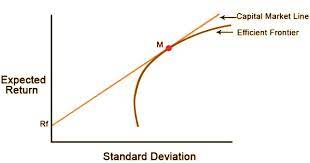
\includegraphics[width=0.5\textwidth]{./imagens/cml.jpg}
                \par \footnotesize Fonte: próprio autor.
                \label{fig:cml}
            \end{figure}


        \paragraph{Equações e fórmulas}
        
        \subparagraph{Exemplo tabela}
            
            \begin{table}[H]
                \centering
                \caption{Tabela inicial do método simplex}
                \begin{tabular}{|c|c|c|c|c|c|c|c|c|}
                    \hline
                            & $z$   & $x_1$ & $x_2$ & $s_1$ & $s_2$ & $s_3$ & $s_4$ & $b$   \\ \hline
                    $z$     & -1    & -3000 & -1000 & 0     & 0     & 0     & 0     & 0     \\ \hline
                    $s_1$   & -     & 1     & 0     & 1     & 0     & 0     & 0     & 6     \\ \hline
                    $s_2$   & -     & 0     & 1     & 0     & 1     & 0     & 0     & 12    \\ \hline
                    $s_3$   & -     & 1     & 1     & 0     & 0     & 1     & 0     & 16    \\ \hline
                    $s_4$   & -     & 1     & $-1/2$& 0     & 0     & 0     & 1     & 2     \\ \hline
                \end{tabular}
                \par \footnotesize Fonte: próprio autor.
                \label{tab:5_4-tabela_inicial}
            \end{table}
        
            e de um quadro:

                        
            \begin{quadro}[H]
                \caption{Restrições do modelo}
                \centering
                \begin{tabular}{|c|c|l|}
                    \hline
                    TIPO                        & Restrição                                     & Descrição                             \\ \hline
                    \multirow{2}{*}{CD}         & \multirow{2}{*}{Capacidade de Expedição}      & O CD possui uma capacidade máxima de  \\
                                                &                                               & expedição de itens em cada turno      \\ 
                    \hline
                    \multirow{17}{*}{Veículos}  & \multirow{4}{*}{Capacidade de Ocupação}       & Cada tipo de veículo possui           \\
                                                &                                               & uma capacidade máxima de ocupação,    \\
                                                &                                               & e pode transportar carga para         \\
                                                &                                               & atender mais de uma loja              \\   \cline{2-3}
                                                & \multirow{3}{*}{Descanso}                     & A cada 12 horas percorridas,          \\
                                                &                                               & o veículo deve permanecer parado      \\
                                                &                                               & por 12 horas para descanso            \\   \cline{2-3}
                                                & \multirow{4}{*}{Custos}                       & Cada tipo de veículo possui           \\
                                                &                                               & um custo fixo por dia de viagem,      \\
                                                &                                               & e um custo variável aplicado à        \\
                                                &                                               & quilometragem percorrida              \\   \cline{2-3}
                                                &                                               & Cada tipo de veículo possui  \\
                                                &                                               & um tempo fixo de carregamento         \\
                                                & Tempo de Carregamento                         & e descarregamento que pode ser        \\
                                                & /Descarregamento                              & adicionado ao tempo de rota           \\
                                                &                                               & independentemente do número           \\
                                                &                                               & de peças transportado                 \\ 
                    \hline
                \end{tabular}
                \label{tab:restricoes}
                \par \footnotesize Fonte: próprio autor.
            \end{quadro}


    \section{SEÇÃO}
        
        \noindent google \cite{Mansini2014}

        \noindent citacao 2 \cite{Markowitz1952}

        \noindent citacao 3 \cite{Vukovic2020}

        \noindent citacao 4 \citeonline{Sharpe1964}.

    \section{CONCLUSÃO}

        \hspace{1.5cm} As conclusões devem responder às questões da pesquisa, em relação aos objetivos e às hipóteses. Devem ser breves, podendo apresentar recomendações e sugestões para trabalhos futuros.

    \section*{REFERÊNCIAS}
        \addcontentsline{toc}{section}{\protect\numberline{}REFERÊNCIAS}
        \renewcommand{\refname}{}
        \bibliography{./referencias/referencias}
        
    \pagebreak
    \appendix
    \section*{APÊNDICE A - Descrição}
        \addcontentsline{toc}{section}{\protect\numberline{}APÊNDICE A - Descrição}
        
    \pagebreak
    \appendix
    \section*{ANEXO A - Descrição}
        \addcontentsline{toc}{section}{\protect\numberline{}ANEXO A - Descrição}

\end{document}